
Commençons par introduire les données fonctionnelles de manière informelle afin de mieux intégrer la définition formelle, plus utile pour la manipulation.

Cette section regroupe l'ensemble des messages essentiels à retenir des données fonctionnelles pour la pratique, sans alourdir les notions avec des notations mathématiques. Le cadre formel sera traité juste après.

\begin{definition*}[données fonctionnelles — informel]
    Les données fonctionnelles sont des données dont les observations sont des fonctions, c'est-à-dire des courbes, des surfaces, des images, \, \dots

    i.e : toute donnée ayant une dépendance de type "relation fonctionnelle" avec un ou plusieurs paramètres.
    \label{def*:fda}
\end{definition*}

\begin{figure}[H]
    \begin{center}
        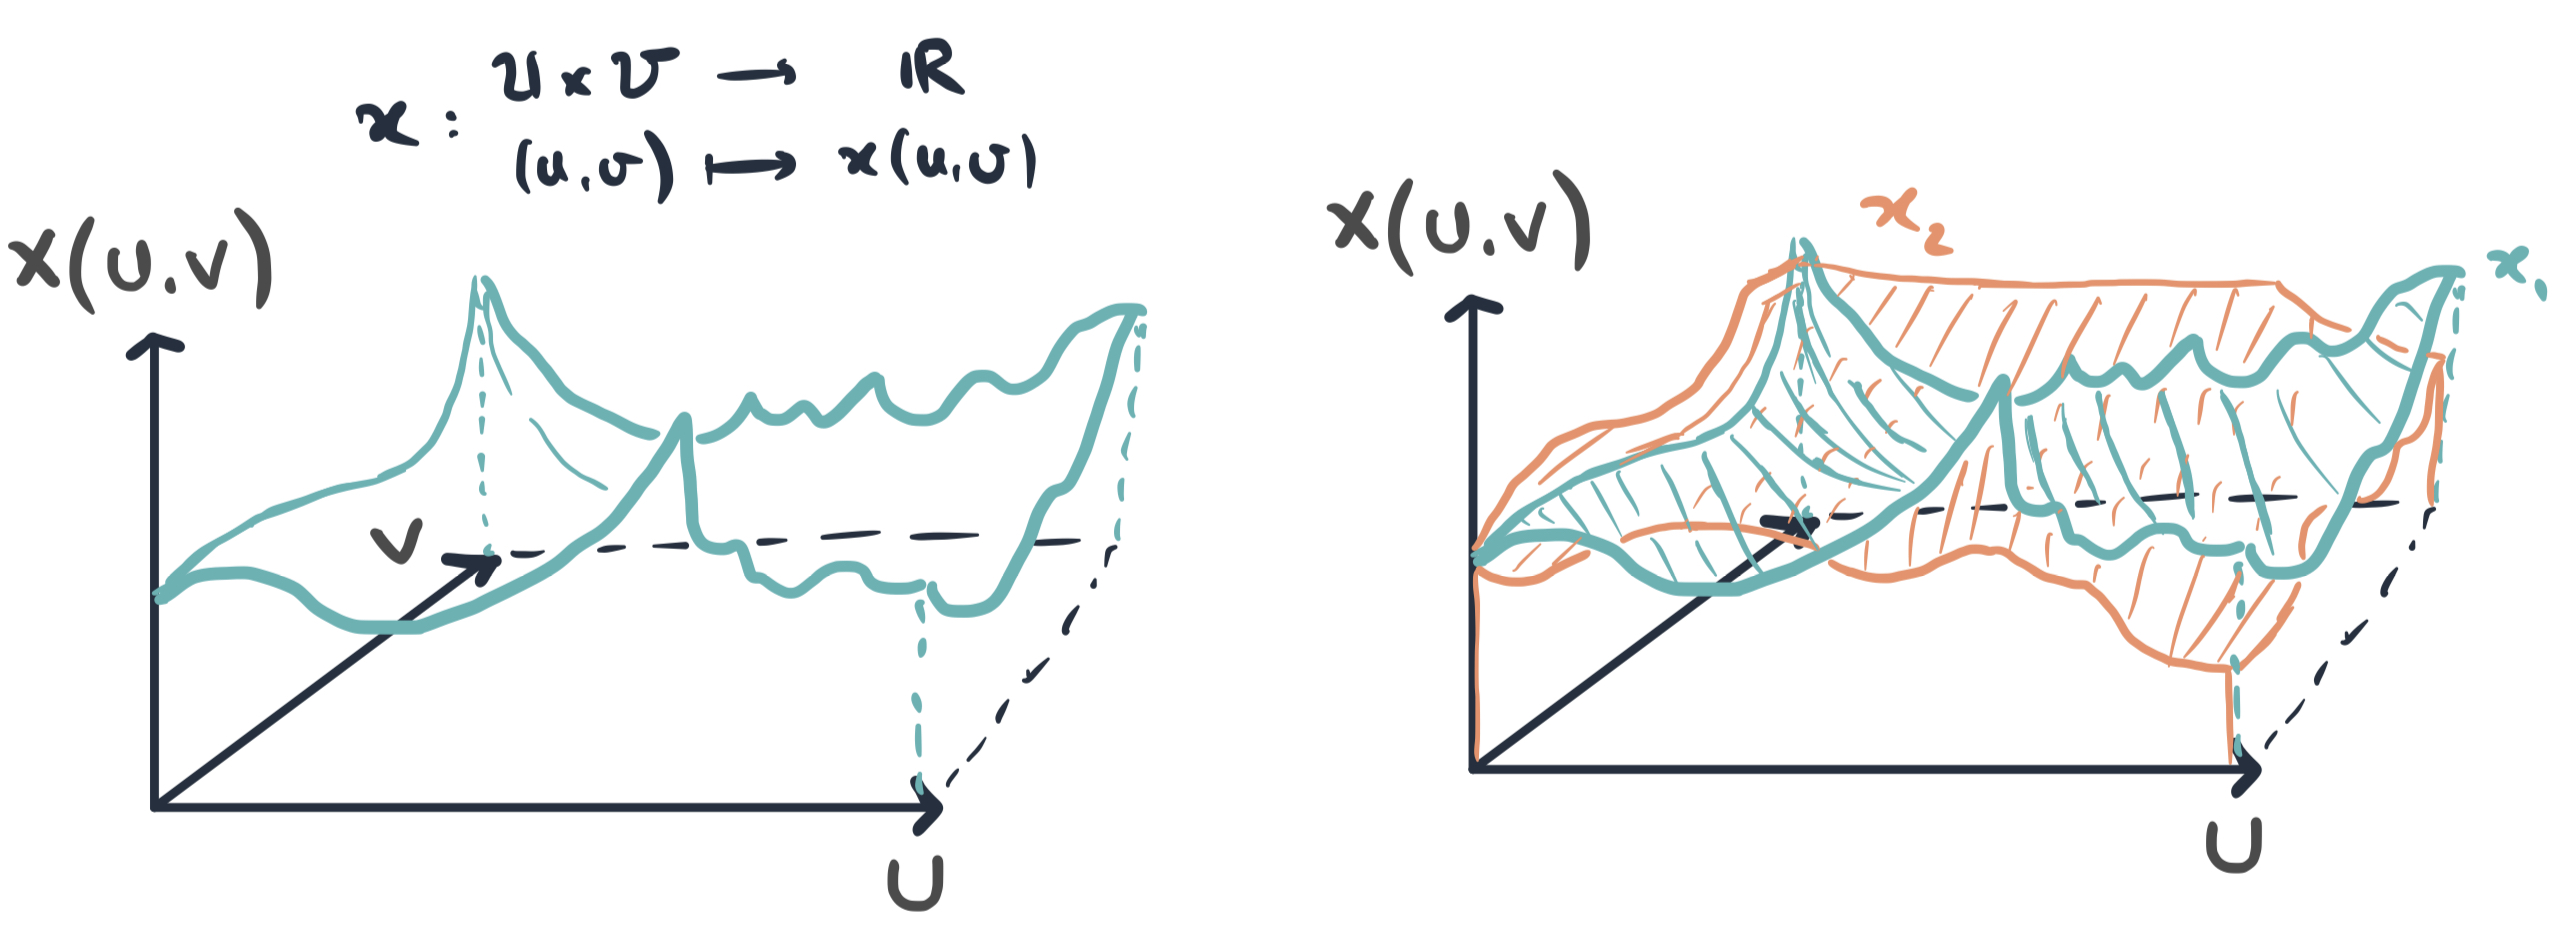
\includegraphics[width=\textwidth]{Images/sketches/fda_surface.jpg}
    \end{center}

    {
    \textbf{Gauche :} exemple de surface
    \\
    \textbf{Droite :} échantillon de deux observations de la surface suivant une loi fonctionnelle}

    \caption{Donnée fonctionnelle : relation fonctionnelle avec plusieurs paramètres}
    \label{fig:sketch_surface}
\end{figure}

Maintenant introduites, les théorèmes suivant permettent de manipuler ces données à la fois pour la théorie et la pratique :

\begin{thm*}[\nameref{thm:KL} — informel]
    \noindent\fbox{%
        \parbox{\textwidth}{%
            Il est possible pour une large classe de données fonctionnelles de les décomposer dans une base \emph{de fonctions} adaptée aux données (au sens de la covariance) que l'on appelle base ACP fonctionelle (FPCA).
        }%
    }
    \label{thm*:KL}
\end{thm*}
\begin{proof}[\faCogs \, preuve informelle]
    La covariance est un opérateur bilinéaire symétrique défini positif, on peut donc appliquer le théorème de Mercer (équivalent du théorème spectral) qui nous donne une base orthonormale de $\mathds L^2$ sur laquelle on va décomposer notre processus \textbf{centré}.
\end{proof}
\begin{rem}
    La classe de fonctions pouvant être décomposées est large, puisqu'elle regroupe l'ensemble des processus qui nous intéressent la plus part du temps en tant que statisticien : celles qui sont à support sur un intervalle, admettant une covariance continue et finie sur le support.
\end{rem}

On en déduit que pour travailler avec des données fonctionnelles, il suffit de les décomposer dans la base ACP fonctionnelle puis de travailler sur les composantes de chaque élément de la base. On travaille désormais avec des réels et non plus des fonctions, ce qu'on aime manipuler. On peut alors faire de la statistique traditionnelle avec les outils que l'on connait.


\begin{propriete*}[intérêt de la base FPCA — informel]
    \noindent\fbox{%
        \parbox{\textwidth}{%
            la base ACP fonctionnelle est la plus économe, c'est à dire qu'elle explique au mieux la covariance des données pour un nombre de composantes fixées, ce qui est utile car on ne sait manipuler numériquement que des objets de dimension finie.
        }%
    }
\end{propriete*}
